\section{Incremental}
The incremental software development methodology is an evolutionary extension 
of the waterfall model \citep{pressman09}. 

The main idea behind this development methodology is that developments are made
in increments, with each increment proving some additional functionality. This
additional functionality often only contains a small progression towards the 
final goal (or product).

Using an incremental approach allows the client to provide feedback, and thus 
the feedback be integrated into the product during development 
\citep{elliott04}. This incremental process continues until the final, 
completed product has been delivered. 

\begin{figure}[H]
  \centering
  \vspace{-80pt}
  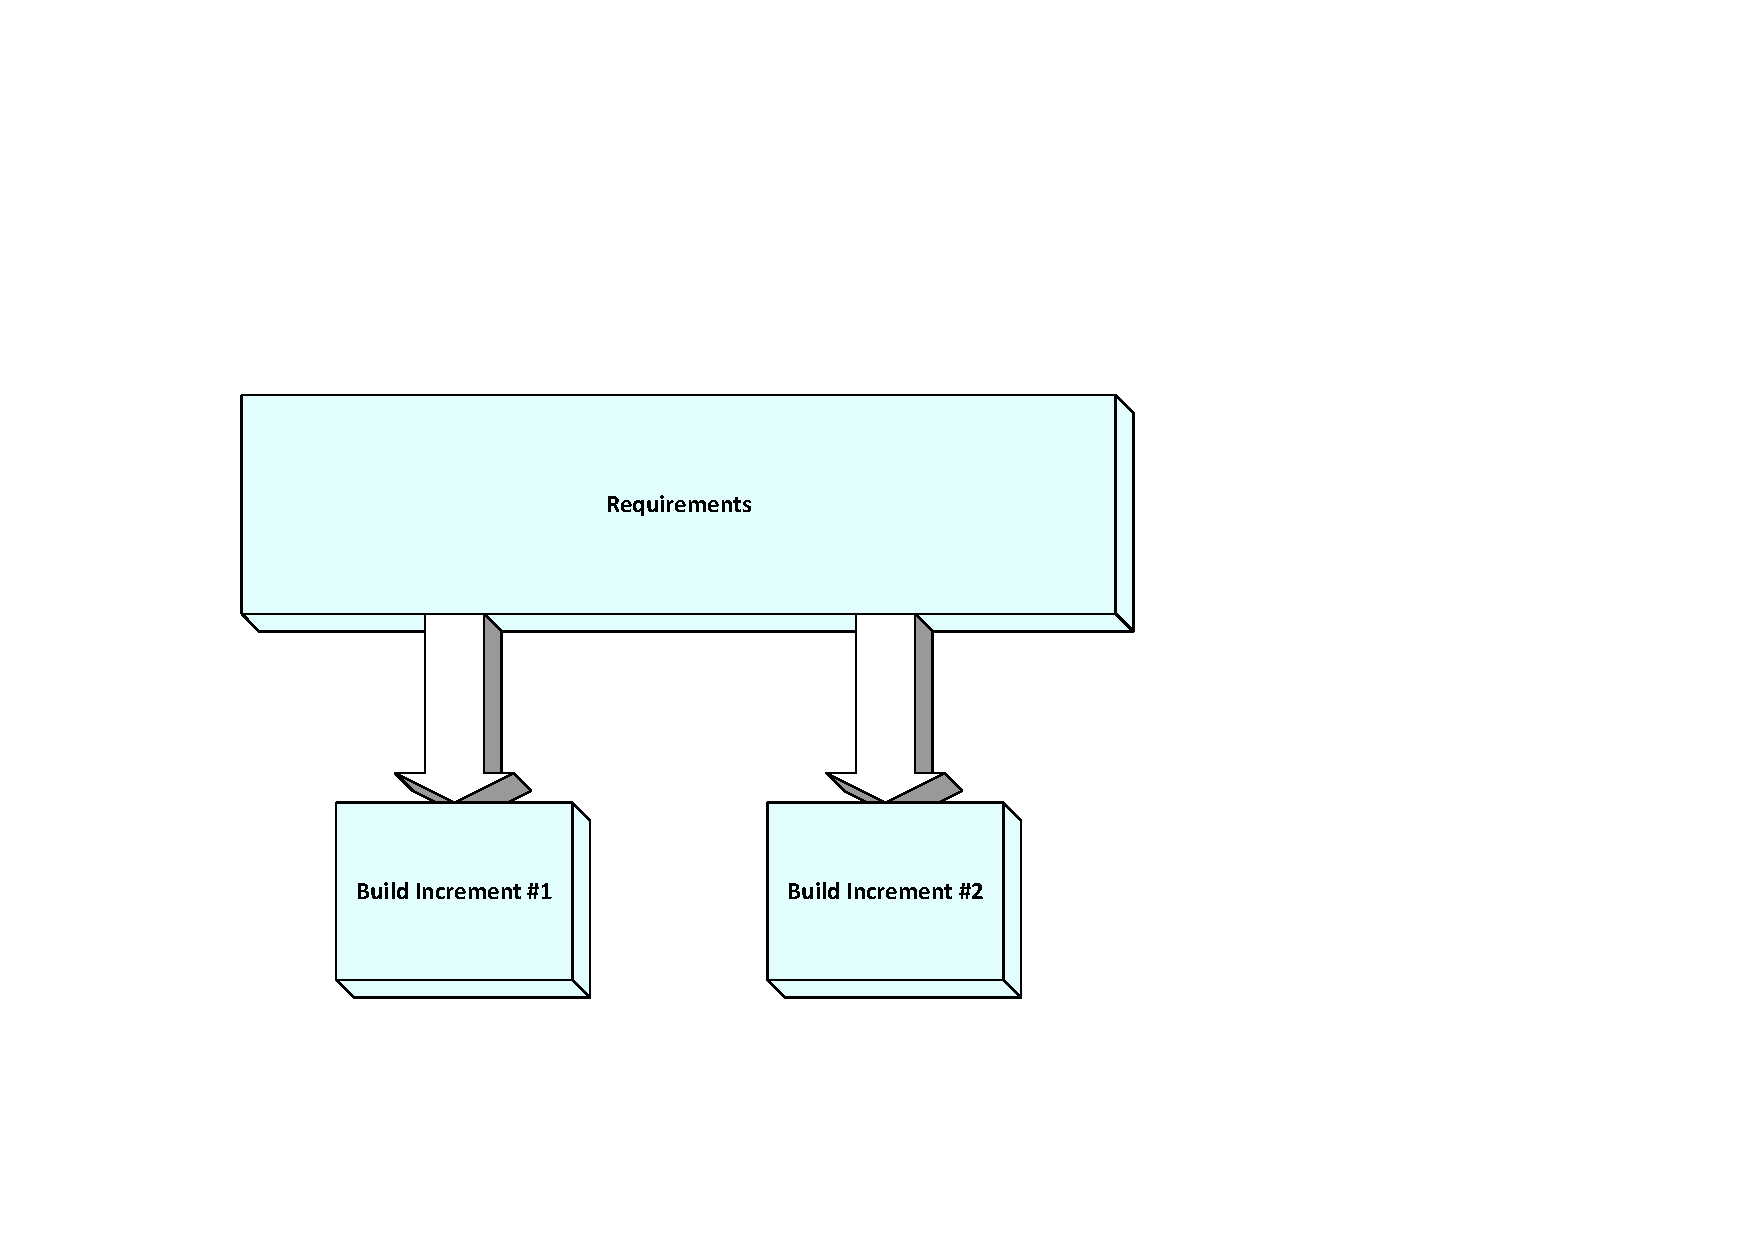
\includegraphics[width=\linewidth]{chapter6/incremental.pdf}
  \vspace{-60pt}
    \caption[Incremental methodology]
      {The incremental methodology allows for the requirements to be segmented 
      into an incremental series of the ``products''.}
\end{figure}

\subsection{Advantages}
The incremental software development methodology could be regarded as having 
the following advantages \citep{elliott04,SDT:2012:Online}:
\begin{itemize}
	\item The user is able to get an early idea of the system's capabilities;
	\item Early and continuous feedback is available from the client;
	\item It allows for more accurate planning, and slippage is easier to spot 
        due to the more frequent deadlines;
	\item It can be easier to test and debug, as any changes that are made within 
        an iteration are small;
	\item The user is able to learn how to use the system ``on the go'' rather 
        than in ``one go''.
\end{itemize}

\subsection{Disadvantages}
There are a number of disadvantages when utilising the incremental software 
development methodology \citep{elliott04,sergei:2012:Online}:
\begin{itemize}
	\item Development can occur for long periods of time, which might exceed the 
        original budget;
	\item Problems related to the system architecture could arise, if additional 
        functionality is added which was not 
				evident in earlier prototypes;
	\item The client may point out too many improvements, which would cause the 
        project to overrun or be completed not meeting the original 
        specification.
\end{itemize}